%! TeX root = relazione.tex

\documentclass{article}

\usepackage[italian]{babel}

\usepackage{listings}             % Scrivere le linee di comando con lsrlisting
\usepackage{graphicx}     % Centrare i testi con center
\usepackage[colorlinks=true, allcolors=blue]{hyperref}  % Link ipertestuali
\usepackage{amsmath}    % Usato per scrivere in linguaggio matematico

% Set page size and margins
% Replace `letterpaper' with `a4paper' for UK/EU standard size
\usepackage[letterpaper,top=2cm,bottom=2cm,left=3cm,right=3cm,marginparwidth=1.75cm]{geometry}

\title{\textbf{KMEANS}}
\author{\textbf{Programmazione di Sistemi Embedded e Multicore}}
\begin{document}
  \maketitle

  \begin{description}
    \centering
    \item \textbf{Nome}: Rideewitage Lachitha Sangeeth 
    \item \textbf{Cognome}: Perera \textbf{Matricola}: 2042904
  \end{description}

  \section{Introduzione}

  Per la parellizzazione del codice sequenziale di KMEANS, sono stati utilizzati due metodi, uno che consiste l'utilizzo di \textbf{OpenMP} insieme a \textbf{OpenMPI},
  e l'altro metodo che utilizza interamente \textbf{CUDA}.
  Prima di analizzare i codici parallelizzati, è necessario capire il funzionamento del codice sequenziale di KMEANS, in quanto sono state apportate delle leggere
  modifiche per il funzionamento dei test.

  
  La prima modifica effettuata al codice sequenziale è stata l'aggiunta di un paramentro in input, che permette di salvare in un file csv il computation time, il quale
  verrà utilizzato per il calcolo della media dei tempi e confrontato con le altre versioni, per la realizzazione di ciò è stata aggiunta anche una funzione che scrive il computation
  time nel file specificato in input [\ref{Write}]. 
  I file contententi i computation times sono salvati in una directory specifica, 
  ovvero: 
  \begin{center}    
    \verb|comp_time/{versione}/comp_time{grandezza_test}.csv|.
  \end{center}
  Oltre a questo, per il corretto funzionamento di tutte le versioni, è stata 
  apportata anche un modifica per quanto riguarda la funzione \verb|eucledianDistance| [\ref{Eucledian}].
  \begin{figure}[ht]
    \hspace{-3cm} % Sposta la figura più a sinistra
    \centering
    \begin{minipage}{0.4\textwidth}
        \centering
        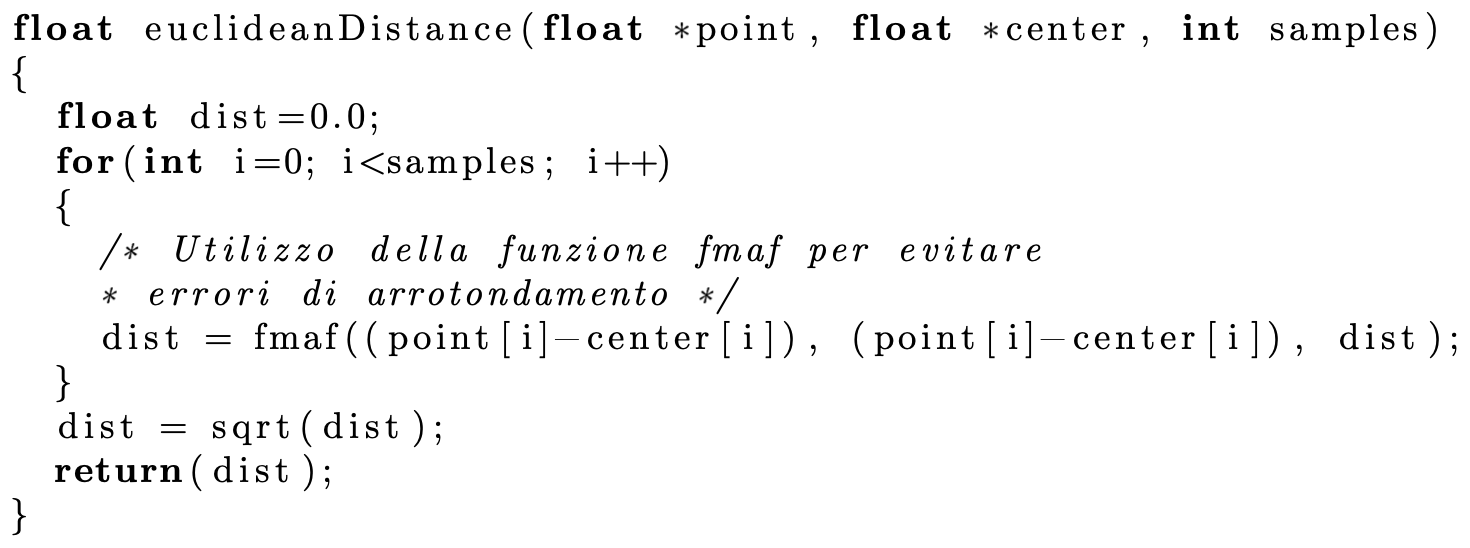
\includegraphics[width=1.5\linewidth]{./Eucledian.png}
        \caption{\textbf{EucledianDistance}}
        \label{Eucledian}
    \end{minipage}
    \hspace{4cm} % Sposta la figura più a sinistra
    \begin{minipage}{0.4\textwidth}
      \centering
      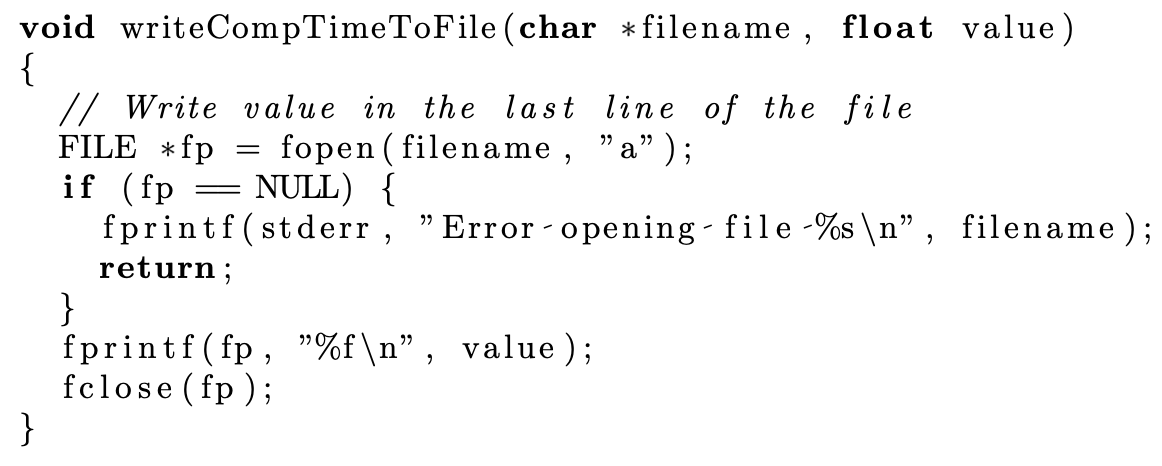
\includegraphics[width=1.4\linewidth]{./Write-Comp.png}
      \caption{\textbf{Write-Comp}}
      \label{Write}
    \end{minipage}
  \end{figure}
  Come è possibile notare dal codice, è stata utilizzata la funzione \verb|fmaf| per evitare possibilie errori
  di arrotondamento; questa modifica è stata apportata in tutte le versioni del codice, questo per fare 
  in modo che la versione ci CUDA non desse output differenti dal sequenziale, in quanto utilizzando la GPU per i calcoli 
  gli arrotondamenti vengono eseguiti in modo diverso rispetto alla CPU. Con l'utlizzo di fmaf, si riduce il numero di arrotondamenti,
  dimnuendo la possibilità di errori.
  \begin{center}
    \rule{6cm}{1pt}
  \end{center}
  Per quanto riguarda il resto del codice, per parallelizzare il codice sequenziale di KMEANS è stato diviso il ciclo \verb|do - while| i tre parti
  fondaemntali, ovvero: 
  \begin{enumerate}
    \item Il reset delle variabili utilizzate ad ogni iterazione [\ref{f_section}]
    \item Il calcolo dei nuovi centroidi e l'assegnazione dei punti ai cluster [\ref{s_section}]
    \item Il calcolo della distanza massima tra i centroidi vecchie e quelli nuovi, per il controllo della threshold impostata dai parametri in input [\ref{t_section}]
  \end{enumerate}
  \begin{figure}[ht]
    \centering
    \begin{minipage}{0.4\textwidth}
        \centering
        \caption{\textbf{First section}}
        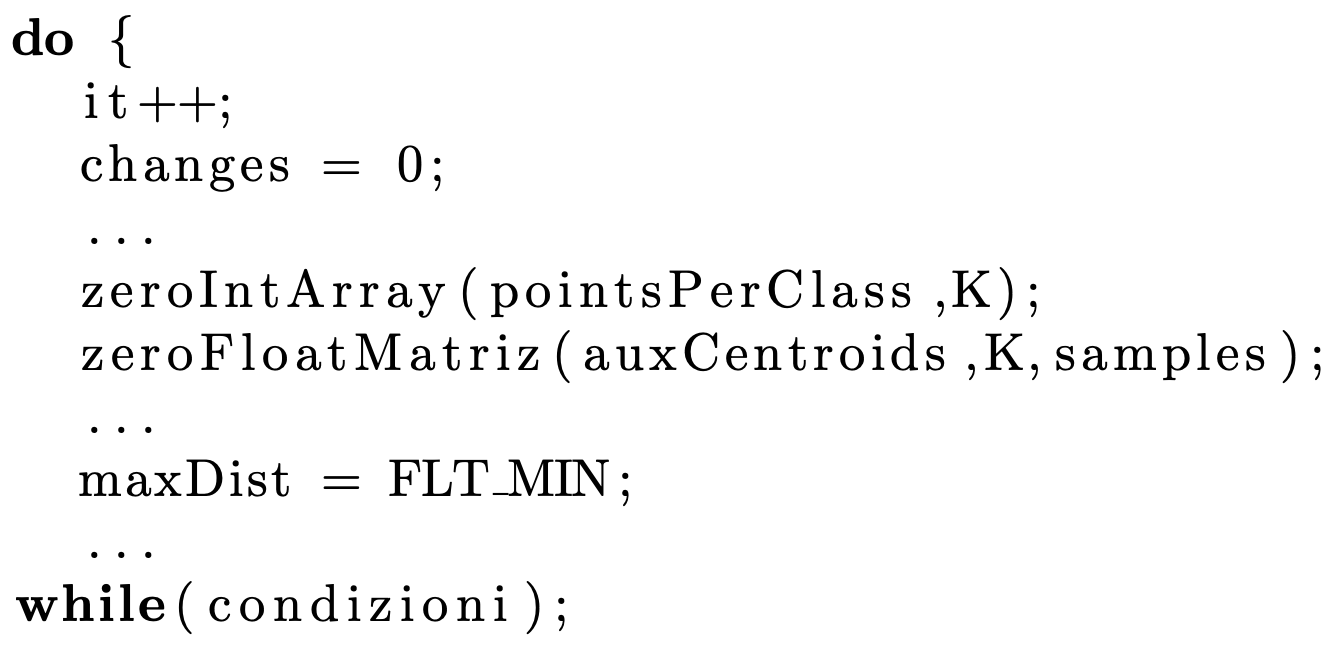
\includegraphics[width=\linewidth]{./First-section.png}
        \label{f_section}
    \end{minipage}
    \begin{minipage}{0.5\textwidth}
        \centering
        \caption{\textbf{Second section}}
        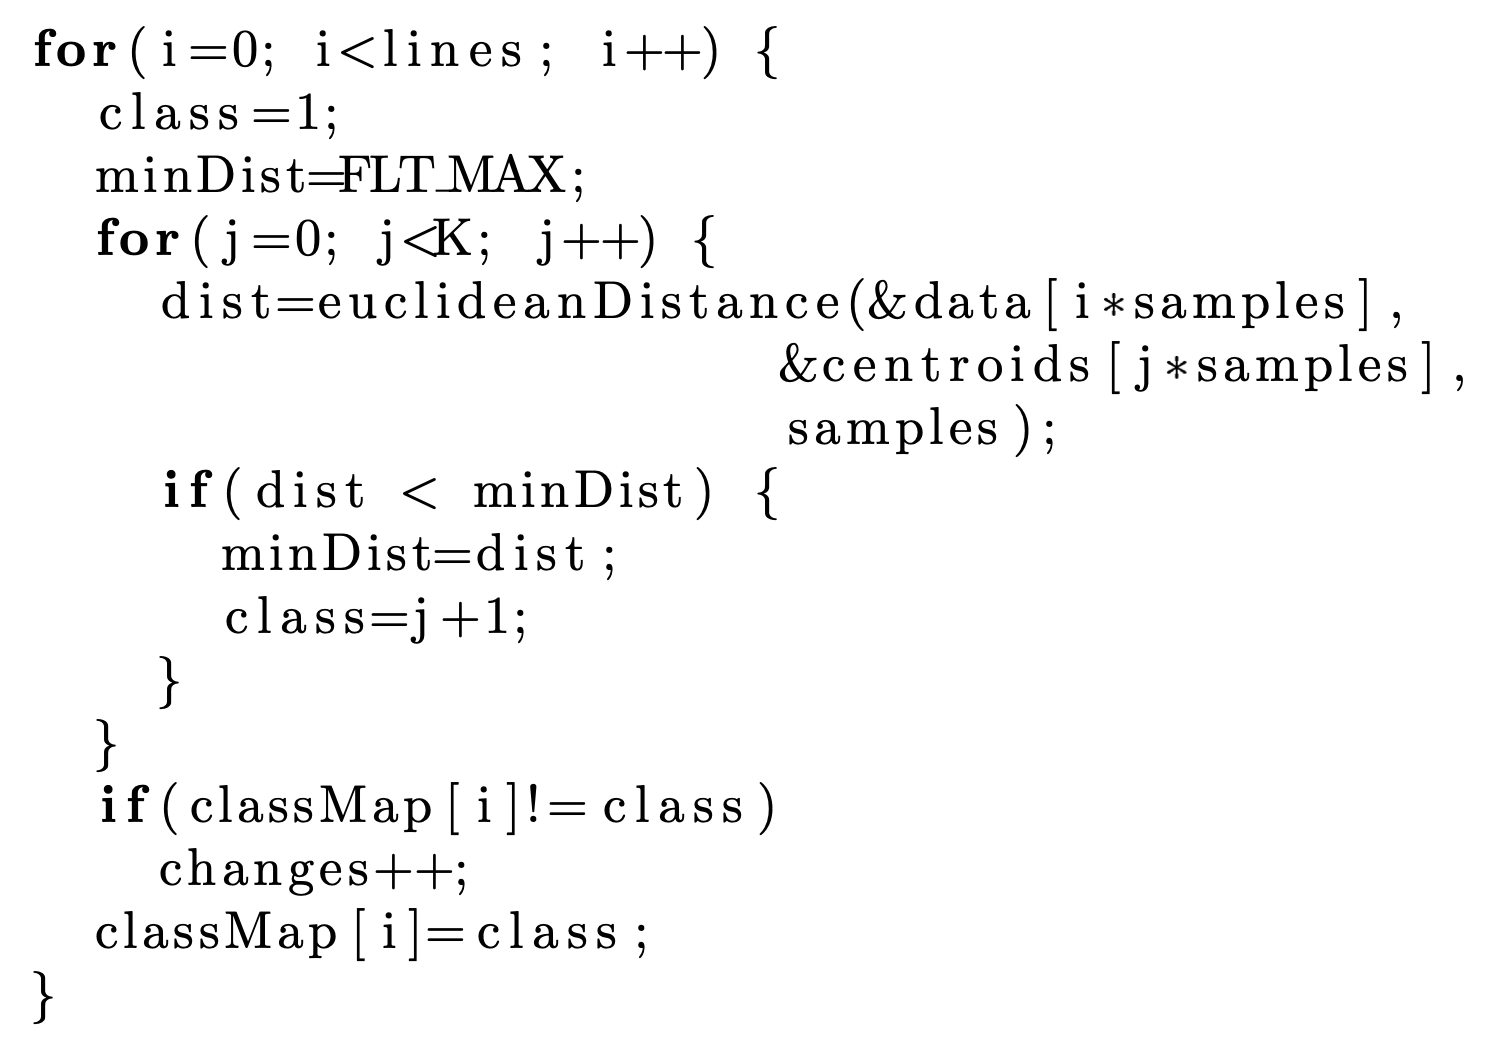
\includegraphics[width=\linewidth]{./Second-section.png}
        \label{s_section}
    \end{minipage}
    \begin{minipage}{0.65\textwidth}
        \centering
        \caption{\textbf{Third section}}
        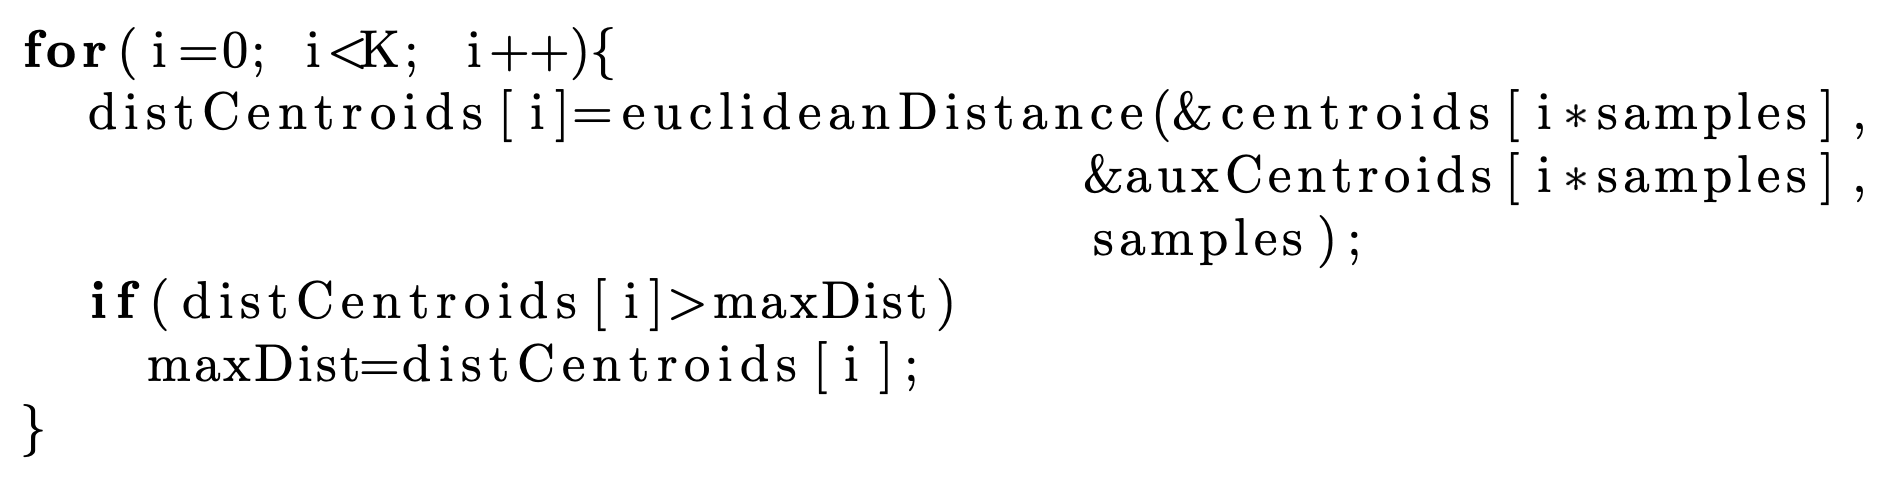
\includegraphics[width=\linewidth]{./Third-section.png}
        \label{t_section}
    \end{minipage}
  \end{figure}
  La parallelizzazione della versione sequenziale, è stata effettuata cercando di parallellizzare le 3 parti appena descritte.
  Oltre a queste parti, è importante anche capire la gestioni dei dati all'interno di ogni iterazione, le variabili 
  che sono state tenute con maggior considerazione durante la parallelizzazione sono: \verb|pointPerClass|, \verb|auxCentroids|,
  \verb|classMap|, \verb|centroids|, \verb|maxDist|, \verb|classMap|.
  \begin{center}
    \rule{6cm}{1pt}
  \end{center}
  Per quanto riguarda \verb|pointPerClass| e \verb|auxCentroids| sono utilizzate per il calcolo dei nuovi centroidi, che è una sezione 
  del codice che non è stata tratta precedentemente, in quanto è stata poi accorpata con la seconda e la terza sezione. In quanto la prima parte 
  del calcolo viene effettuata su un ciclo che itera sul numero di linee (come la seconda sezione), mentre la seconda parte del colcolo viene effettuata 
  su un ciclo che itera sul numero di cluster (come la terza sezione).
  
  La variabile \verb|classMap| riporta per ogni dato passato dal file di input il cluster a cui viene assegnato. Il contenuto di questa variabile 
  viene poi trascritta con la funzione \verb|writeResult(filename)| sul file passato in input (specificata negli argomenti utilizzando il seguente path:
  \begin{center}
    \verb|output_files/{versione}/output{grandezza_test}.txt|).
  \end{center}
  Invece, la variabile \verb|centroids| rappresenti i centroidi attuali, i quali all'inizio vengono generati randomicamente, in seguito, dopo la prima iterazione del ciclo
  \verb|do - while| viene sovrascritto da \verb|auxCentroids| controllando che la distanza massima di cambiamento, ovvero \verb|maxDist|, sia minore della massima distanza specificata
  negli argomenti.

  \subsection{Check validity and Testing script}

  Per quanto riguarda l'esecuzione dei test e il controllo della validità di un'esecuzione sono stati creati due script python (\verb|tester.py| e \verb|run.py|) all'interno della cartella \verb|py_prog/|.
  \begin{center}
    \rule{2.5cm}{1pt} \makebox{\texttt{run.py}} \rule{2.5cm}{1pt}
  \end{center}
  Il file \verb|run.py| viene utilizzato per l'esecuzione di un singolo test, impostato il file \verb|.sub| per il submit del job sul cluster in base alla versione che si vuole eseguire (MPI + OMP, CUDA o sequenziale). 
  Una volta eseguito il test, per controllare la correttezza dell'output generato controllo il contenuto del file con il file di output generato dalla versione sequenziale.
  Per quanto riguarda il setting del file job sono state create 3 funzioni, una per versione, in cui in ognuna modifica il file \verb|.sub| della propria versione all'interno della directory \verb|jobs/| impostando 
  tutti i settagi necessari per l'esecuzione del test (per esempio il file di input, dove salvare l'output e il computation time, nel caso di MPI + OMP il numero di thread e di processi).
  \begin{center}
    \rule{2.5cm}{1pt} \makebox{\texttt{tester.py}} \rule{2.5cm}{1pt}
  \end{center}
  Per quanto rifuarda l'esecuzione dei test per il calcolo dell'Avarage Time, è stato creato un'altro script python, ovvero, il file \verb|tester.py| il quale utilizza
  la libreria \verb|unittest| per l'esecuzione dei test in tutte e tre le versioni. I test vengono eseguiti attraverso la funzione main importata da \verb|run.py|; ogni singolo 
  test viene ripetuto 50 volte, per avere dei dati più precisi per quanto riguarda l'AvgTime.
  Dopo l'esecuzione dei test esegue il calcolo dell'AvgTime del test e viene salvato su un file \verb|{versione}.csv| in cui ogni riga ha il seguente formato: 
  \begin{center}
    \verb| Number of Process, Number of Thread, AvgTime Test 2D2, ..., AvgTime Test 100D2 |  
  
    \small *Nel caso del sequenziale e di CUDA il numero di processi e thread è 0
  \end{center}

  \section{CUDA Version}

  Per la versione CUDA sono state implementate due funzioni kernel, che rappresentato due delle sezioni spiegate nell'introduzione (Figure: \ref{s_section} e \ref{t_section}), e 3 variabili \verb|__costant__| che sono
  il numero di cluster, linee e samples. Per ogni chiamata ad una funzione cuda è stata usata \verb|CHECK_CUDA_CALL| per verificare se la funzione passata in input ha generato un errore.
  Come prima modifica, è sono state agigunte nella sezione di allocazione della memoria (nella funzione \verb|main|) le funzioni \verb|cudaMalloc| e \verb|cudaMemcpy| per l'allocazione della memoria sulla GPU e il trasferimento dei dati dalla CPU alla GPU per ogni
  variabile utilizzata all'interno delle funzioni kernel, mentre, per le variabili \verb|__costant__| è stata usata la funione \verb|cudaMemcpyToSymbol|.
  
  In seguito all'allocazione della memoria e allo spostamento delle variabili, e prima del ciclo \verb|do| - \verb|while|, 
  vengono impostati le dimensioni di ogni blocco e i thread per blocco in base al numero di linee (determinato dal file di input) e cluster (determinato dal parametro passato in input).
  \begin{lstlisting}[language=C]
    dim3 blockSize(1024);
    dim3 numBlocks(ceil(static_cast<double>(lines) / blockSize.x));
    dim3 numBlocks2(ceil(static_cast<double>(K) / blockSize.x));
  \end{lstlisting}
  Come si nota viene utilizzata la funzione \verb|ceil()| per evitrare che non vengano scartate le ultime iterazioni.
  \begin{center}
    \rule{2.5cm}{1pt} \makebox{\texttt{Kernel Functions}} \rule{2.5cm}{1pt}
  \end{center}
  All'interno del ciclo \verb|do| - \verb|while| vengono inzialmente reimpostate (attraverso la funzione \verb|cudaMemset|) le seguenti variabili: \verb|d_changes|, \verb|d_maxDist|, \verb|d_pointPerClass|, \verb|d_auxCentroids|.
  Inseguito al reset delle variabili vengono chiamati i due kernel. Il primo definito nel seguente modo:
  \begin{enumerate}
    \item Definizione della funzione kernel:
      \begin{lstlisting}[language=C, xleftmargin=-5em]
        __global__ void assign_centroids(float* d_data, float* d_centroids, 
                        int* d_classMap, int* d_changes, int* d_pointsPerClass,
                        float* d_auxCentroids)
      \end{lstlisting}
      La funzione viene utilizzata per assegnare ogni punto del file in input al cluster più vicino, e calcolare il numero di punti per ogni cluster e aumenta 
      il numero di cambiamenti per iterazione (ricordiamo che il numero di cambiamenti viene resettato ad ogni iterazione del ciclo) se un punto cambia di cluster. Inseguito
      inizia il calcolo dei nuovi centroidi, che conclude con il secondo kernel.
    \item Inizalmente la funzione calcola l'indice del thread e controlla se il thread è minore del numero di linee:
      \begin{lstlisting}[language=C, xleftmargin=-5em]
        int id = (blockIdx.x * blockDim.x) + threadIdx.x;
        if (id < d_lines)
      \end{lstlisting}
    \item All'interno dell'\verb|if| viene eseguita la seconda sezione [\ref{s_section}], lavorando con le variabili che si trovano nella GPU, spostati precedentemente dalla CPU nella sezione 
      dell'allocazione della memoria.
  \end{enumerate}
  Questa implementazione del kernel è stata fatta per parallelizzare il calcolo dei nuovi centroidi e l'assegnazione dei punti ai cluster più vicini.

\end{document}
